
\chapter[Suporte Tecnológico]{Suporte Tecnológico}\label{ch:suporteTecnologico}
  Esse capítulo irá apresentar as principais tecnologias e ferramentas envolvidas no desenvolvimento deste trabalho.
  Desse modo, este  capítulo está dividido nas seções: Unity 3D (\ref{sub:unity3D}), Kinect (\ref{sub:kinect}) e Ferramentas (\ref{sub:solFerramentas}).

  \section{Unity 3D}\label{sub:unity3D}

      O Unity 3D é uma ferramenta, criado para jogos em três e duas dimensões, além de ser
    multiplataforma. Com ênfase na portabilidade ele tem como alvo o maior número
    de APIs gráficas possíveis, desde o sistema operacional da microsoft, o windows,
    ao android.  Tem suporte para programação em C\# e JavaScript. O unity 3D também
     possui uma licença pessoal, livre de custo \cite{unity3D}.

      Para a criação de um produto acessível, o matlab não seria viável pois
      sua licença é paga e ele é geralmente usado para prototipação. Com isso foi usado o Unity 3D, um motor gráfico muito usado na indústria de software para desenvolvimento de jogos comerciais e livres.

    \section{Kinect}\label{sub:kinect}
      O kinect é um sensor de movimentos, desenvolvido inicialmente para as plataformas
    de jogos eletrônicos da microsoft. Ele possui uma camara RGB (\textit{Red, Green, Blue}),
    um sensor de profundidade, um microfone embutido, e a versão mais recente, chamado de kinect 2.0,
    consegue detectar 25 articulações esqueletais por pessoa \cite{{microsoftResearch}}.

    \begin{figure}[H]
    \centering
    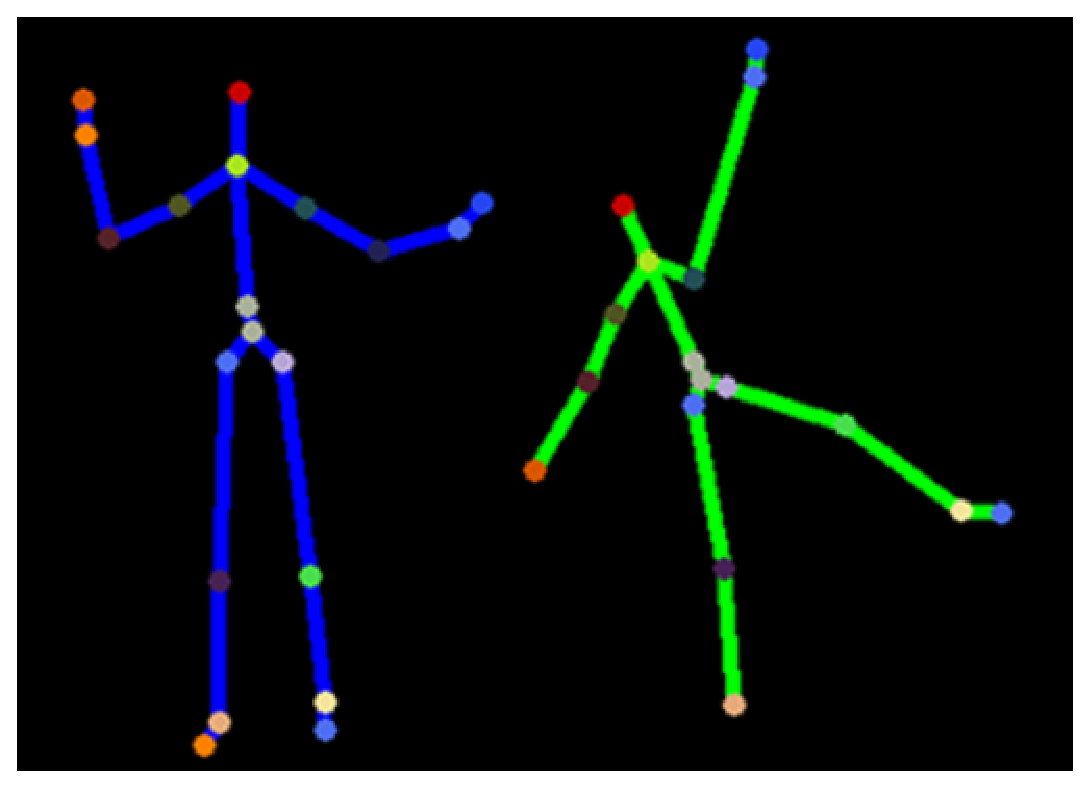
\includegraphics [keepaspectratio=true,scale=0.60]{figuras/esqueletoKinect.eps}
    \caption{Esqueleto Kinect. Fonte: \cite{microsoftResearch}.}

    \label{esqueletokinect}
    \end{figure}

    \subsection{\textit{kinect for windows SDK V1.8 }}\label{sub:sdk}
      O \textit{kinect for windows SDK V1.8}, fornece ferramentas e APIs necessários para desenvolver
    aplicações Kinect nas linguagens  C++, C\#, Visual Basic, ou outra linguagem .NET. Hoje em sua versão 2.0,
    entre seus recursos estão o acesso completo ao Kinect: vídeo,
    profundidade, áudio, motor e funções de alto nível e também  criar aplicativos
    para o sistema operacional da microsoft e seu console para jogos.

     O SDK é necessário, pois o sistema operacional reconhece o sensor, permitindo aos
     desenvolvedores criar aplicativos que suportem o uso do kinect, e disponibiliza a comunicação com o Unity3D.

      Além disso, o SDK envolve uma variedade
    de classes e métodos com algoritmos já produzidos e disponibilizados para utilização
    durante o desenvolvimento. Com a utilização da SDK, o desenvolvedor não se preocupa
    com a implementação de algoritmos comuns, como a obtenção de dados dos
    sensores.

    A tecnologia Unity3D é multiplataforma, possibilitando sua utilização em vários Sistemas operacionais
    porém o SDK é somente suportado no windows.

    \section{Ferramentas}\label{sub:solFerramentas}
      Para o desenvolvimento do sistema foram usadas diversas ferramentas, a seguir serão apresentadas junto
    dos artefatos gerados.

    \subsection{GIT}\label{sub:git}
      A ferramenta GIT\footnote{https://git-scm.com/} foi desenvolvida por Linus Torvalds, mesmo criador do Linux,
    sendo uma ferramenta \textit{open-source}. Disponibiliza uma eficiente forma de versionamento de códigos e
    gerenciamento de projetos.

    \subsection{Github}\label{sub:github}
      O Github\footnote{https://github.com} é uma ferramenta utilizada para hospedagem remota de projetos GIT.
    Neste trabalho o Github foi utilizado para hospedar a versão escrita do documento e pode ser acessado \href{https://github.com/ricardogtx/Tcc}{aqui}\footnote{https://github.com/ricardogtx/Tcc}.

    \subsection{Gitlab}\label{sub:gitlab}
      O Gitlab\footnote{https://gitlab.com} é outra ferramenta utilizada para hospedagem remota de projetos GIT.
       Esta ferramenta foi utilizada para hospedar o código e pode ser acessado
    \href{https://gitlab.com/ricardogtx/Tcc}{aqui}\footnote{https://gitlab.com/ricardogtx/Tcc}.

    \subsection{Linux Debian}\label{sub:linuxdebian}
    		O sistema operacional utilizado durante este trabalho é o Linux Debian\footnote{https://www.debian.org/} sistema livre
    e utilizado, neste projeto, para documentação do trabalho.

    \subsection{Windows}\label{sub:windows}
    Sistema operacional da Microsoft 10\footnote{https://www.microsoft.com/pt-br/} , utilizado para implementação do código
    por possibilitar configuração simplificada da comunicação entre o \textit{Kinect} e o computador.

     \subsection{Visual Studio}\label{sub:codigo}
       Para a edição e criação do código foi usado o Micorosoft Visual Studio\footnote{https://www.visualstudio.com/pt-br/} uma IDE\textit{(Integrated development enviroment)} disponibilizada pela microsoft
    e possui apoio para várias linguagens de programação, principalmente C\#.

    \subsection{Atom}\label{sub:atom}
    		O Atom\footnote{https://atom.io/} é um editor de texto, possui apoio para diversas linguagens de programação, incluindo textos em LaTeX, além de
    ter um núcleo hackeável e muito configurável.



    \subsection{Astah community}\label{sub:diagramaSequencia}
      É um software para modelagem uml - Linguagem de Modelagem Unificada, neste trabalho esta ferramenta foi usado para criação do diagrama de sequências, que consiste em um diagrama que tem o objetivo de mostrar como as mensagens entre os objetos são trocadas no decorrer do tempo para a realização de uma operação\cite{diagramaSequencia}.

    Como pode ser visto em \ref{diagramaFisio} e \ref{diagramaPaciente}, existe dois momentos de trocas de mensagens, uma com o usuário como fisioterapeuta e outra
    como paciente. A ferramenta Astah community pode ser encontrada aqui\footnote{http://astah.net/download}.


    \subsection{\textit{Trello}}\label{sub:trello}
      Ao longo do desenvolvimento foi utilizado o \textit{trello}\footnote{https://trello.com/}  que é uma espécie de \textit{kanban eletrônico} (\ref{sec:kanban}).
